%%%%%%%%%%%%%%%%%%%%%%%%%%%%%%%%%%%%%%%%%%%%%%%%%%%%%%%%%%%%%
%  PREAMBLE: sets up compiler modes, loads packages, defines macros, etc
%%%%%%%%%%%%%%%%%%%%%%%%%%%%%%%%%%%%%%%%%%%%%%%%%%%%%%%%%%%%%

%%%%%%%%%%%%%%%%%%%%%%%%%%%%%%%%%%%%%%%%%%%%%%%%%%%%%%%%%%%%%
%  PREAMBLE: sets up compiler modes, loads packages, defines macros, etc
%  Steve Rodney, 2012
%%%%%%%%%%%%%%%%%%%%%%%%%%%%%%%%%%%%%%%%%%%%%%%%%%%%%%%%%%%%%


%%%%%%%%%%%%%%%%%%%%
% COMPILER MODES
%%%%%%%%%%%%%%%%%%%%

%% Set default compiler modes 
%% (these will be overridden by the -options.tex  file below, if it exists)

% Manuscript mode : 
%  True  : single-column, double-spaced, markup-ready style (with comments)
%  False : print in two-col single-space publication-ready style (no comments)
\newif\ifms
\msfalse

% Grayscale  mode : use grayscale figures when available
\newif{\ifgrayscale}
\grayscalefalse

% Changetext mode : highlight modified text in bold blue font
\newif{\ifchangetext}
\changetextfalse

%% Read in the -options.tex file (generated by the Makefile)
%%  to set the compile-mode options
\InputIfFileExists{\jobname-options}


%%%%%%%%%%%%%%%%%%%%%%%%%%%%%%%
% manuscript mode settings
%%%%%%%%%%%%%%%%%%%%%%%%%%%%%%%
\ifms
  \documentclass[manuscript]{aastex}
  \usepackage{natbib,amsmath,verbatim}
  \received{}
  \revised{}
  \accepted{}
  \citestyle{aa}
  \newcommand{\cmt}[1]{\textcolor{red}{#1}}   % Red text  for printing comments 
\else
  %\documentclass[12pt,ms,iop]{emulateapj}
  \documentclass[revtex4,iop]{emulateapj}
  \font\sevenrm=cmr7 
  \citestyle{aa} 
  \newcommand{\cmt}[1]{}
  %\slugcomment{submitted to ApJ} 
  %\journalinfo{astro-ph/xxxxxx}  % top left corner of first page.
\fi

%%%%%%%%%%%%%%%%%%%%%%%%%%%%%%%
% changetext  mode settings
%%%%%%%%%%%%%%%%%%%%%%%%%%%%%%%
\ifchangetext
  % Changed text is highlighted in bold, blue font 
  \newcommand{\change}[1]{{\bf \textcolor{blue}{#1}}}
\else
  % Changed text is indistinguishable
  \newcommand{\change}[1]{#1}
\fi


%%%%%%%%%%%%%%%%%%%%
% PACKAGES INCLUDED
%%%%%%%%%%%%%%%%%%%%
\usepackage{natbib}   % reference citations and bibliography
\usepackage{amsmath}  % extended math symbols
\usepackage{verbatim} % verbatim text formatting
\usepackage{enumerate}% enumerated lists
\usepackage{amssymb}  % extended symbols lib
%\usepackage{url}      % url text formatting
\usepackage{hyperref}      % url text formatting
\usepackage[usenames]{color}  % colored text
%\usepackage{multirow}  % muti-row table cells
%\usepackage{amsmath}  % extended equations lib (split)
%\usepackage{mathrsfs} % extended math fonts (mathscr)
%\usepackage{paralist} % inline enumeration (for Table ref lists)
%\usepackage{authblk}
\usepackage{appendix}


%%%%%%%%%%%%%%%%%%%%%%%%%%%%%%%%%%%%%%%%%%%%%%%%%%%
% PDF mode settings : Auto-select eps or pdf figures 
% based  on the compiler used (i.e. latex vs pdflatex)
%%%%%%%%%%%%%%%%%%%%%%%%%%%%%%%%%%%%%%%%%%%%%%%%%%%
\ifx\pdfoutput\undefined
  \pdffalse
  \DeclareGraphicsExtensions{.eps,.ps}
\else
  \ifnum\pdfoutput=1
    % \pdftrue
    \DeclareGraphicsExtensions{.pdf,.png,.jpg}
  \else
    % \pdffalse
    \DeclareGraphicsExtensions{.eps,.ps}
  \fi
\fi


%%%%%%%%%%%%%%%%%%%%%%%%%%%%%%%
% AUTHOR-DEFINED MACROS
%%%%%%%%%%%%%%%%%%%%%%%%%%%%%%%

% Paper aliases 
\defcitealias{Patel:2014}{P14}
\def\P14{\citetalias{Patel:2014}}

\def\tomas{HFF14Tom}

% General purpose usefulness:
\newcommand{\etal}{{et al.~}}                                             
\def\eg{{e.g.}}
\def\ie{{i.e.}}
\def\etc{{etc.}}
\newcommand{\lta}{\lesssim}                                               
\newcommand{\gta}{\gtrsim}                                                
\newcommand{\gt}{\gtsim}
\newcommand{\kms}{\,\rm km\,s^{-1}}                                       


%\def\pmstat{ \ensuremath{ \substack{ \resizebox{0.7em}{0.5em}{$\pm$} \\ \resizebox{0.7em}{0.2em}{stat}} } }
\def\pmstat{\ensuremath{\substack{\pm \\ \mbox{\scalebox{0.45}{stat}} } } }
\def\pmsyst{\ensuremath{\substack{\pm \\ \mbox{\scalebox{0.45}{syst}} } } }

% Cosmology:
\def\Om{\ensuremath{\Omega_{\rm m}}}
\def\Ot{\ensuremath{\Omega_{\rm tot}}}
\def\Ob{\ensuremath{\Omega_{\rm b}}}
\def\OL{\ensuremath{\Omega_{\Lambda}}}
\def\Ok{\ensuremath{\Omega_{\rm k}}}
\def\om{\ensuremath{\omega_{\rm m}}}
\def\ob{\ensuremath{\omega_{\rm b}}}
\def\wo{\ensuremath{w_0}}
\def\wa{\ensuremath{w_{\rm a}}}
\def\lcdm{$\Lambda$CDM}
\def\LCDM{$\Lambda$CDM}
\def\wcdm{$w$CDM}
\def\Ho{\ensuremath{H_0}}
\def\DA{\ensuremath{D_A}}
\def\DL{\ensuremath{D_L}}

% Astronomy:
\def\arcsec{\ensuremath{^{\prime\prime}}} 
\def\kms{\ensuremath{{\rm km s}^{-1}}}
\def\hgpcq{\mbox{$h^{-3}$Gpc$^3$}}
\def\hmpcq{\mbox{$h^{-3}$Mpc$^3$}}
\def\perhmpcq{\mbox{$h^{3}$Mpc$^{-3}$}}
\def\hmpc{\mbox{$h^{-1}$Mpc}}
\def\hmpci{\mbox{$h$\,Mpc$^{-1}$}}
\def\mpc{\mbox{Mpc}}
\def\mpci{\mbox{Mpc$^{-1}$}}
\def\mpcq{\mbox{Mpc$^{-3}$}}
\def\Msun{\mbox{M$_{\odot}$}}
\def\Av{\mbox{$A_V$}}
\def\Rv{\mbox{$R_V$}}

% Supernovae : 
\newcommand{\CCSN}{CC\,SN}
\newcommand{\CCSNe}{CC\,SNe}
\newcommand{\TNSN}{TN\,SN}
\newcommand{\TNSNe}{TN\,SNe}
\newcommand{\SNIa}{SN\,Ia}
\newcommand{\SNeIa}{SNe\,Ia}
\newcommand{\SNRz}{SNR($z$)}
\def\Mch{\mbox{M$_{\rm Ch}$}}
\def\Ni{\ensuremath{^{56}\mbox{Ni}}}
\newcommand{\dmfifteen}{\ensuremath{\Delta\mbox{m}_{15}}}
\newcommand{\deltamfifteen}{\ensuremath{\Delta\mbox{m}_{15}}}

% Missions:
\def\Hubble{{\it Hubble}}
\def\Hubbles{{\it Hubble's}}
\def\Spitzer{{\it Spitzer}}
\def\Chandra{{\it Chandra}}
\def\Herschel{{\it Herschel}}
\def\XMM{{\it XMM}}

% Institutions
\newcommand{\JHU}{Department of Physics and Astronomy, The Johns Hopkins University, Baltimore, MD 21218.}
\newcommand{\elsewhere}{St. Elsewhere University.}
\newcommand{\STScI}{Space Telescope Science Institute, Baltimore, MD 21218.}
\newcommand{\Berkeley}{Department of Astronomy, University of California, Berkeley, CA 94720-3411.}
\newcommand{\Riverside}{Department of Physics and Astronomy, University of California, Riverside, CA 92521.}
\newcommand{\WKU}{Department of Physics, Western Kentucky University, Bowling Green, KY 42101.}
\newcommand{\Copenhagen}{Dark Cosmology Centre, Niels Bohr Institute, University of Copenhagen, Juliane Maries Vej 30, DK-2100 Copenhagen, Denmark.}
\newcommand{\Arizona}{Department of Astronomy, University of Arizona, Tucson, AZ 85721.}
\newcommand{\SantaCruz}{Department of Astronomy and Astrophysics, University of California, Santa Cruz, CA 92064.}
\newcommand{\NotreDame}{Department of Physics, University of Notre Dame, Notre Dame, IN 46556.}
\newcommand{\TelAviv}{Department of Astrophysics, Tel Aviv University, 69978 Tel Aviv, Israel.}
\newcommand{\Rutgers}{Department of Physics and Astronomy, Rutgers, The State University of New Jersey, Piscataway, NJ 08854.}
\newcommand{\CfA}{Harvard/Smithsonian Center for Astrophysics, Cambridge, MA 02138.}
\newcommand{\Minnesota}{Department of Astronomy, University of Minnesota, 116 Church Street SE, Minneapolis, MN 55455, USA.}


%%%%%%%%%%%%%%%%%%%%%%%%%%%%%%%
% Page Setup 
%%%%%%%%%%%%%%%%%%%%%%%%%%%%%%%
\ifms
\else
  \renewcommand{\topfraction}{0.9}
  \renewcommand{\bottomfraction}{0.9}
  \renewcommand{\textfraction}{0.1}
  \renewcommand{\floatpagefraction}{0.9}
  \renewcommand{\dbltopfraction}{0.9}
  \renewcommand{\dblfloatpagefraction}{0.9}
\fi



%%%%%%%%%%%%%%%%%%%%%%%%%%%%%%%%%%%%%%%%%%%%%%%%%%%%%%%%%%%%
% MAIN DOCUMENT TEXT
%%%%%%%%%%%%%%%%%%%%%%%%%%%%%%%%%%%%%%%%%%%%%%%%%%%%%%%%%%%%

\shorttitle{A Type Ia SN Behind Abell 2744}
\shortauthors{Rodney et al.}

\begin{document}

\title{Illuminating a Dark Lens : A Type Ia Supernova Magnified by Galaxy Cluster Abell 2744}

\author{
 Steven~A.~Rodney\altaffilmark{1},
  \etal
}
\altaffiltext{1}{\JHU}
\altaffiltext{2}{Hubble fellow}



\begin{abstract}
SN \tomas\ is a Type Ia Supernova (\SNIa) discovered at $z=1.33$
behind the galaxy cluster Abell 2744 ($z=0.308$). This SN has a
projected separation from the cluster core of $\sim$40\arcsec, closer
than any other cluster-lensed \SNIa.  As such, it provides the first
opportunity to confront gravitational lens models of galaxy clusters
with the direct measurement of an absolute magnification at the edge
of the strong-lensing region.  We derive a tightly constrained measure
of the peak apparent magnitude, corrected for light curve shape and
exinction.  In a cosmology-independent analysis, we find that \tomas\
is $0.71\pm0.12$ magnitudes brighter than unlensed \SNeIa\ at similar
redshift, implying a lensing magnification of $\mu_{\rm
obs}=1.9\pm0.2$.  Predicted magnifications from 7 independent groups
are systematically biased to higher values, with a mean of $\mu_{\rm
mod}=2.4\pm0.3$ and some models disagreeing by $>6\sigma$.  
\textcolor{red}{TODO: summarize lensing discussion.}
%The most
%significant discrepancies arise from models with a strict ``light
%traces mass'' assumption.  We evaluate possible causes for this bias,
%including variation of the mass-to-light ratio in the nearest cluster
%member galaxy.  A sample of \textcolor{red}{$\sim$10??} \SNeIa\ behind
%any single cluster could provide a robust evaluation of systematic
%biases in lens models.  Until such a sample exists, it is advisable to
%increase the estimated uncertainty of any predicted magnification
%by an amount comparable to the dispersion from all available lens
%models.

\end{abstract}

\keywords{ supernovae: general }

\section{Introduction}
\label{sec:Introduction}

Massive galaxy clusters can be used as cosmic telescopes to magnify
distant background objects through gravitational lensing.  This can
substantially increase the reach of deep imaging surveys, and has
recently been used to discover candidate proto-galaxies formed in the
first Gyr after the Big
Bang \citep{Zheng:2012,Coe:2013} 
\textcolor{red}{(cite other high-z galaxy candidates discovered with lensing)}

Lensed SNe have been discovered
\citep{Goobar:2009,Riehm:2011,Patel:2014,Nordin:2014}

In Section~\ref{sec:DiscoveryAndFollowup} we present the discovery and
follow-up observations of SN \tomas at $z=1.31$, discovered behind the
galaxy cluster Abell 2744.  Sections~\ref{sec:Spectroscopy} and \ref{sec:PhotometricClassification}
describe the spectroscopy and photometry of this SN, leading to a
classification of the object as a normal Type Ia SN.  In
Section~\ref{sec:LensingMagnification} we make a direct measurement of
the magnification of this source due to gravitational lensing, and
compare to predicitions from lens models.  Finally,
Section~\ref{sec:Discussion} discusses the tension between our
magnification measurement and the lens models, with implications for
the systematic error budget in magnification estimates for other
high-$z$ lensed sources.


\section{Discovery, Follow-up, and Data Processing}
\label{sec:DiscoveryAndFollowup}

\begin{figure*}
\begin{center}
%\includegraphics[width=\textwidth]{FIG/discovery_image}
\includegraphics[width=\textwidth]{FIG/discovery_image_lowres}
\caption{  \label{fig:DiscoveryImage} 
SN \tomas\ in the Abell 2744 field.  The left panel shows a
UV/Optical/IR color composite image constructed from all available HST
imaging of the Abell 2744 cluster field.  The inset panels at right
show F814W imaging of the immediate vicinity of SN \tomas,
approximately 40\arcsec\ from the center of the cluster. The top panel
shows the template image, combining all data prior to the SN
appearance.  Labeled ellipses mark the nearest galaxies and their
redshift constraints: a photometric redshift for the most likely host
galaxy is marked in blue, and the spectroscopic redshift for a likely
background galaxy is given in yellow. The bottom panel is constructed
from all HFF F814W imaging taken while the SN was detectable, and
marks the SN location with an arrow.  (Left panel image credit: NASA,
ESA, and J. Lotz, M. Mountain, A. Koekemoer, and the HFF Team (STScI))
}
\end{center}
\end{figure*}


SN \tomas\ was discovered in \HST\ observations with the Advanced
Camera for Surveys (ACS) in the F606W and F814W bands (V and i),
collected on UT 2014 May 15 as part of the Hubble Frontier Fields
(HFF) survey (PI:J.Lotz,
HST-PID:13495).\footnote{\url{http://www.stsci.edu/hst/campaigns/frontier-fields}}
The HFF program is a 3-year director's discretionary initiative that
is collecting 140 orbits of HST imaging (roughly 340 ksec) on six
massive galaxy clusters, plus 6 accompanying ``parallel fields.''
Each field is observed in 3 optical bands (ACS F435W, F606W and F814W)
and 4 infrared (IR) bands (WFC3-IR F105W, F125W, F140W, and F160W),
although the optical and IR imaging campaigns are separated by $\sim$6
months. Abell 2744 was the first cluster observed, with IR imaging
spanning 2013 October-November, and optical imaging from 2014
May-July.  A composite image of the HFF data showing the SN is
presented in Figure~\ref{fig:DiscoveryImage}.  The SN detection was
made in difference images constructed using template imaging of Abell
2744 from HST+ACS observations taken in 2009 (PI:Dupke,
HST-PID:11689).

\begin{deluxetable*}{rrlrrlrlcc}
\tablecolumns{9}
\tablecaption{\tomas\ Observations and Photometry\label{tab:Photometry}}
\tablehead{ 
    \colhead{Obs. Date}
  & \colhead{Camera}
  & \colhead{Filter}
  & \colhead{Exp. Time}
  & \colhead{Flux}
  & \colhead{Flux Err}
  & \colhead{AB Mag\tablenotemark{a}}
  & \colhead{Mag Err}
  & \colhead{AB Zero Point} 
  & \colhead{$\Delta$ZP\tablenotemark{b}} \\
    \colhead{(MJD)}
  & \colhead{}
  & \colhead{or grism}
  & \colhead{(sec)}
  & \colhead{(counts/sec)}
  & \colhead{(counts/sec)}
  & \colhead{}
  & \colhead{}
  & \colhead{} 
  & \colhead{(Vega-AB)} 
}
\startdata
56820.1 & ACS     & F435W &   5083 &   -0.149 & 0.288 &  27.66 &  \nodata  &   25.665 & -0.102\\
56821.9 & ACS     & F435W &   5083 &    0.568 & 0.287 &  28.12 &     0.55  &   25.665 & -0.102\\
56823.8 & ACS     & F435W &   5083 &    0.120 & 0.286 &  29.80 &     2.58  &   25.665 & -0.102\\
56825.0 & ACS     & F435W &   5083 &    0.115 & 0.288 &  29.85 &     2.72  &   25.665 & -0.102\\
56828.7 & ACS     & F435W &   5083 &   -0.801 & 0.289 &  27.66 &  \nodata  &   25.665 & -0.102\\
56830.9 & ACS     & F435W &   5083 &    0.544 & 0.290 &  28.16 &     0.58  &   25.665 & -0.102\\
56832.9 & ACS     & F435W &   5083 &   -0.431 & 0.288 &  27.66 &  \nodata  &   25.665 & -0.102\\
56833.9 & ACS     & F435W &   5083 &   -0.011 & 0.285 &  27.67 &  \nodata  &   25.665 & -0.102\\
56839.5 & ACS     & F435W &   5083 &   -0.118 & 0.282 &  27.68 &  \nodata  &   25.665 & -0.102\\[1mm]
56792.1 & ACS     & F606W &   5046 &    0.917 & 0.210 &  27.59 &     0.25  &   26.493 & -0.086\\
56793.0 & ACS     & F606W &   3586 &    1.750 & 0.240 &  26.89 &     0.15  &   26.493 & -0.086\\
56797.1 & ACS     & F606W &   4977 &    2.447 & 0.221 &  26.53 &     0.10  &   26.493 & -0.086\\
56800.1 & ACS     & F606W &   4977 &    2.134 & 0.215 &  26.68 &     0.11  &   26.493 & -0.086\\
56805.0 & ACS     & F606W &   5046 &    2.471 & 0.218 &  26.52 &     0.10  &   26.493 & -0.086\\[1mm]
56793.0 & ACS     & F814W &   3652 &    6.851 & 0.433 &  25.41 &     0.07  &   25.947 & -0.424\\
56797.1 & ACS     & F814W &   4904 &   14.111 & 0.589 &  24.63 &     0.05  &   25.947 & -0.424\\
56799.0 & ACS     & F814W &   5046 &   16.515 & 0.654 &  24.46 &     0.04  &   25.947 & -0.424\\
56800.1 & ACS     & F814W &   4904 &   16.111 & 0.647 &  24.48 &     0.04  &   25.947 & -0.424\\
56801.9 & ACS     & F814W &  10092 &   17.147 & 0.641 &  24.42 &     0.04  &   25.947 & -0.424\\
56803.0 & ACS     & F814W &  10092 &   18.080 & 0.670 &  24.36 &     0.04  &   25.947 & -0.424\\
56803.9 & ACS     & F814W &  15138 &   18.401 & 0.670 &  24.34 &     0.04  &   25.947 & -0.424\\
56804.1 & ACS     & F814W &   5046 &   19.470 & 0.746 &  24.28 &     0.04  &   25.947 & -0.424\\
56812.1 & ACS     & F814W &    637 &   19.666 & 1.078 &  24.27 &     0.06  &   25.947 & -0.424\\
56815.9 & ACS     & F814W &    446 &   16.831 & 1.190 &  24.45 &     0.08  &   25.947 & -0.424\\
56820.1 & ACS     & F814W &   5044 &   14.663 & 0.595 &  24.58 &     0.04  &   25.947 & -0.424\\
56821.9 & ACS     & F814W &   5044 &   14.802 & 0.600 &  24.57 &     0.04  &   25.947 & -0.424\\
56823.8 & ACS     & F814W &   5044 &   12.021 & 0.518 &  24.80 &     0.05  &   25.947 & -0.424\\
56825.0 & ACS     & F814W &   5044 &   12.792 & 0.539 &  24.73 &     0.05  &   25.947 & -0.424\\
56828.7 & ACS     & F814W &   5044 &   11.609 & 0.506 &  24.84 &     0.05  &   25.947 & -0.424\\
56830.9 & ACS     & F814W &   5044 &   10.013 & 0.462 &  25.00 &     0.05  &   25.947 & -0.424\\
56832.9 & ACS     & F814W &   5044 &    9.743 & 0.453 &  25.03 &     0.05  &   25.947 & -0.424\\
56833.9 & ACS     & F814W &   5044 &    9.987 & 0.462 &  25.00 &     0.05  &   25.947 & -0.424\\
56839.5 & ACS     & F814W &   5044 &    6.993 & 0.390 &  25.39 &     0.06  &   25.947 & -0.424\\[1mm]
56833.1 & WFC3-IR & F105W &    756 &   23.317 & 0.742 &  24.10 &     0.09  &   26.269 & -0.645\\
56841.8 & WFC3-IR & F105W &    756 &   18.090 & 0.648 &  24.40 &     0.11  &   26.269 & -0.645\\
56850.1 & WFC3-IR & F105W &    756 &   12.281 & 0.643 &  24.77 &     0.12  &   26.269 & -0.645\\
56860.6 & WFC3-IR & F105W &   1159 &    9.008 & 0.520 &  25.13 &     0.12  &   26.269 & -0.645\\
56886.6 & WFC3-IR & F105W &   1159 &    3.779 & 0.458 &  26.09 &     0.22  &   26.269 & -0.645\\
56891.7 & WFC3-IR & F105W &    356 &    3.018 & 1.007 &  26.34 &     0.34  &   26.269 & -0.645\\
56893.2 & WFC3-IR & F105W &    712 &    2.965 & 0.753 &  26.33 &     0.32  &   26.269 & -0.645\\
56954.6 & WFC3-IR & F105W &    356 &    1.618 & 1.206 &  27.01 &     0.65  &   26.269 & -0.645\\[1mm]
56817.1 & WFC3-IR & F125W &   1206 &   27.248 & 0.615 &  23.92 &     0.06  &   26.230 & -0.901\\
56833.2 & WFC3-IR & F125W &    756 &   24.972 & 0.822 &  24.01 &     0.06  &   26.230 & -0.901\\
56841.8 & WFC3-IR & F125W &    806 &   19.374 & 0.733 &  24.29 &     0.07  &   26.230 & -0.901\\
56850.1 & WFC3-IR & F125W &    806 &   13.989 & 0.722 &  24.64 &     0.09  &   26.230 & -0.901\\[1mm]
56891.9 & WFC3-IR & F140W &    712 &    6.770 & 0.903 &  25.42 &     0.19  &   26.452 & -1.076\\
56893.1 & WFC3-IR & F140W &    712 &    9.551 & 0.868 &  25.06 &     0.14  &   26.452 & -1.076\\
56955.6 & WFC3-IR & F140W &   1424 &    3.199 & 0.707 &  26.25 &     0.23  &   26.452 & -1.076\\[1mm]
56817.1 & WFC3-IR & F160W &   1206 &   20.211 & 1.102 &  24.27 &     0.09  &   25.946 & -1.251\\
56833.2 & WFC3-IR & F160W &    756 &   16.591 & 1.007 &  24.46 &     0.10  &   25.946 & -1.251\\
56841.8 & WFC3-IR & F160W &    756 &   12.599 & 0.978 &  24.76 &     0.10  &   25.946 & -1.251\\
56850.1 & WFC3-IR & F160W &    756 &   11.482 & 0.933 &  24.86 &     0.13  &   25.946 & -1.251\\
56860.7 & WFC3-IR & F160W &   1159 &    7.927 & 0.740 &  25.26 &     0.16  &   25.946 & -1.251\\
56886.6 & WFC3-IR & F160W &   1159 &    7.018 & 0.800 &  25.40 &     0.16  &   25.946 & -1.251\\[1mm]
\tableline\\
56812.0 & ACS     & G800L &   3490 &  \nodata & \nodata & \nodata & \nodata & \nodata & \nodata\\
56815.7 & ACS     & G800L &   6086 &  \nodata & \nodata & \nodata & \nodata & \nodata & \nodata
\enddata
\tablenotetext{a}{For non-positive flux values we report the magnitude as a 3-$\sigma$ upper limit}
\tablenotetext{b}{Zero point difference: the magnitude shift for conversion from AB to Vega magnitude units.}
\end{deluxetable*}






\begin{figure}
\begin{center}
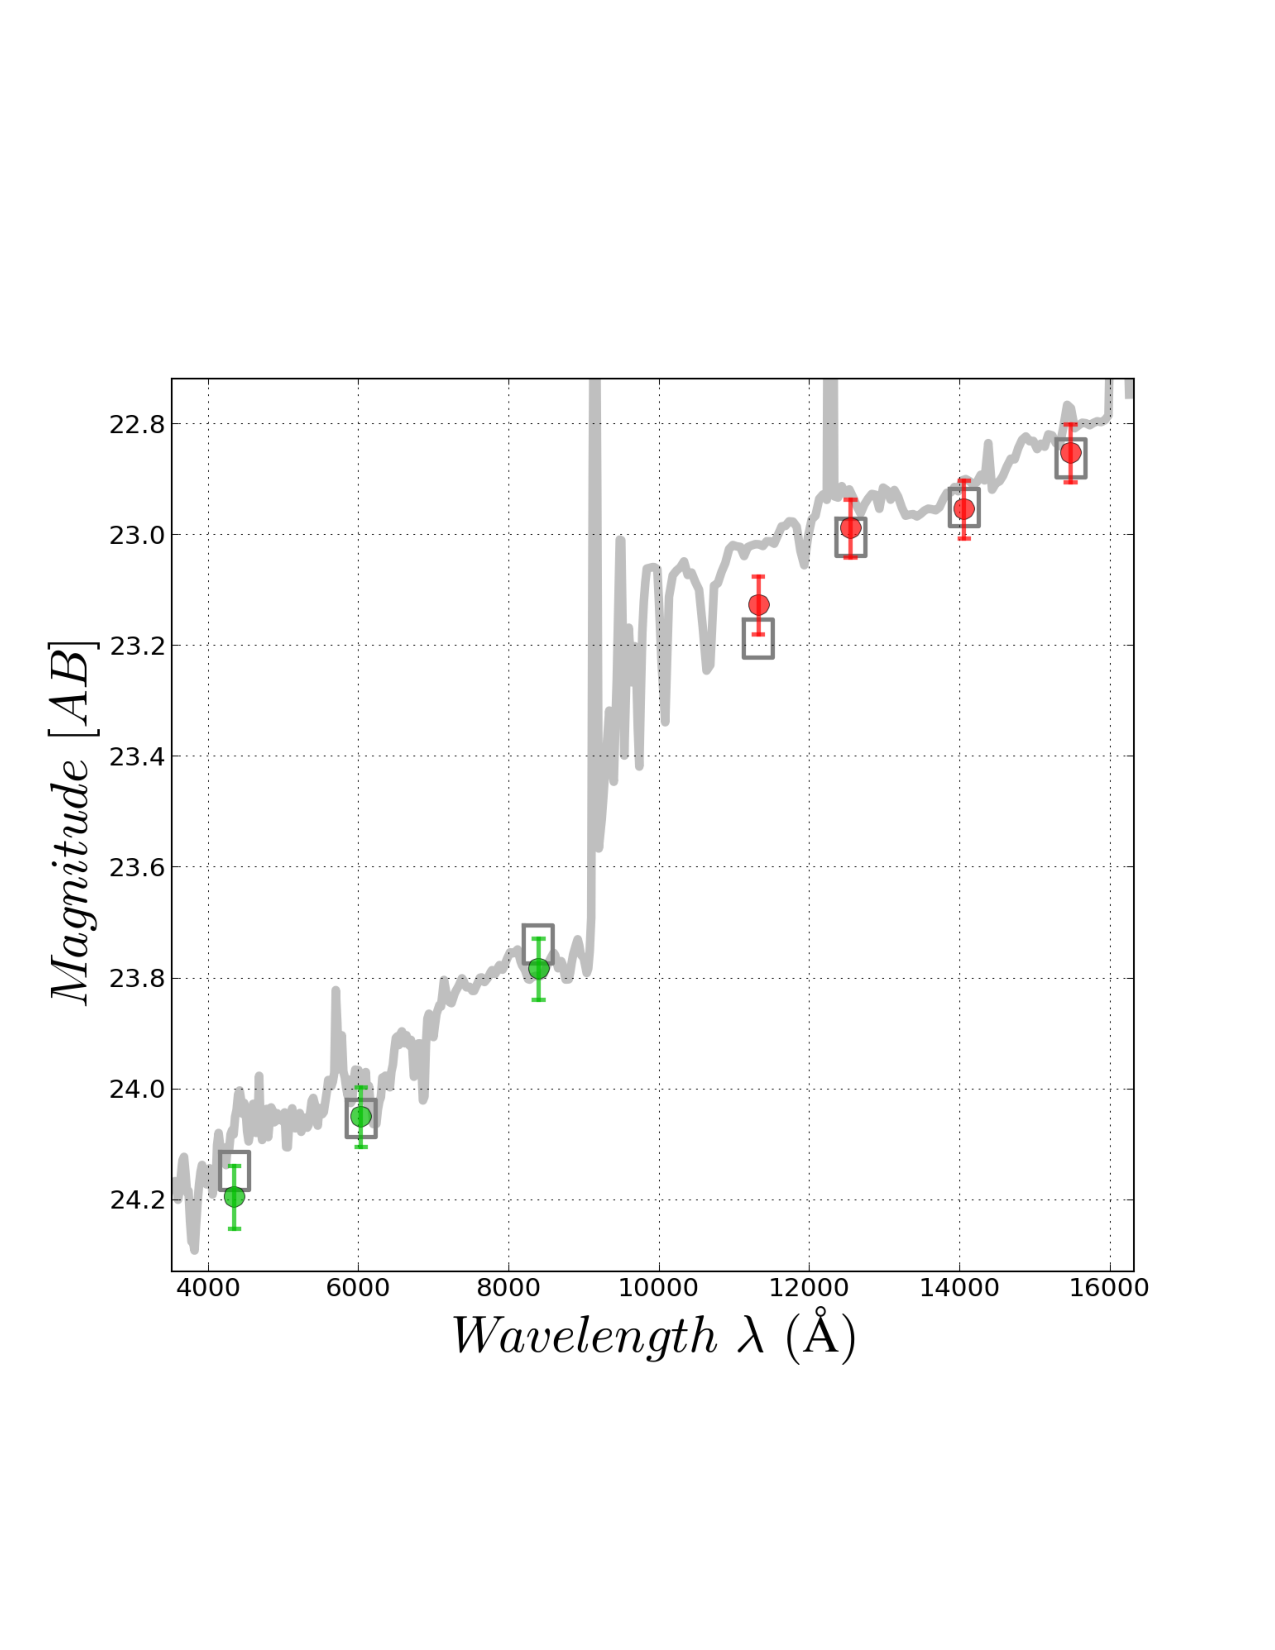
\includegraphics[width=\columnwidth]{FIG/host_sed_fit}
\caption{  \label{fig:HostSED}
Best-fit SED template match for the most probable \tomas\ host
galaxy. Using the {\it BPZ} code to match the observed SED, we find
the nearest galaxy to the SN position is a late type galaxy with a
photometric redshift of $z=1.5\pm0.2$.}
\end{center}
\end{figure}

The most probable host galaxy for SN \tomas\ is a faint and diffuse
galaxy immediately to the south-east of the SN location.  With
photometry of the host galaxy collected from the template images, we
fit the spectral energy distribution (SED) using the {\it BPZ} code --
a Bayesian photometric redshift estimator \citep{Benitez:2000}. The best-fit
SED template match is shown in Figure~\ref{fig:HostSED}.  From the
{\it BPZ} analysis, we found the host to be most likely a late-type
galaxy at a redshift of $z=1.5\pm0.2$.  

Upon discovery, HST target-of-opportunity
observations were triggered from the FrontierSN program (PI:Rodney,
HST-PID:13386), which aims to discover and follow transient sources in
the HFF cluster and parallel fields. The FrontierSN observations
provided WFC3-IR imaging as well as spectroscopy using the ACS G800L
grism, supplementing the rapid-cadence optical imaging from HST+ACS
already being provided by the HFF program. Difference images for the
IR follow-up data were generated using templates constructed from the
HFF WFC3-IR imaging campaign, which concluded in November, 2013.

All of the imaging data were processed using the {\tt sndrizpipe}
pipeline,\footnote{\url{https://github.com/srodney/sndrizpipe} v1.2
DOI:10.5281/zenodo.10731} a custom data reduction package in Python
that is employs the {\tt DrizzlePac} tools from the Space Telescope
Science Institute (STScI) \citep{Fruchter:2010}.  Photometry was
collected using the {\tt PyPhot} software
package,\footnote{\url{https://github.com/djones1040/PyPhot}} a
pure-Python implementation of the photometry algorithms from the IDL
AstroLib package \citep{Landsman:1993}, which in turn are based on the
DAOPHOT program \citep{Stetson:1987}.  For the IR bands we used point
spread function (PSF) fitting on the difference images, and in the ACS
optical bands we collected photometry with a
0\farcs3 aperture. Table~\ref{tab:Photometry} presents the list of
observations, along with measured photometry from all available
imaging data.
 


\section{Spectroscopy}
\label{sec:Spectroscopy}

\begin{figure}
\begin{center}
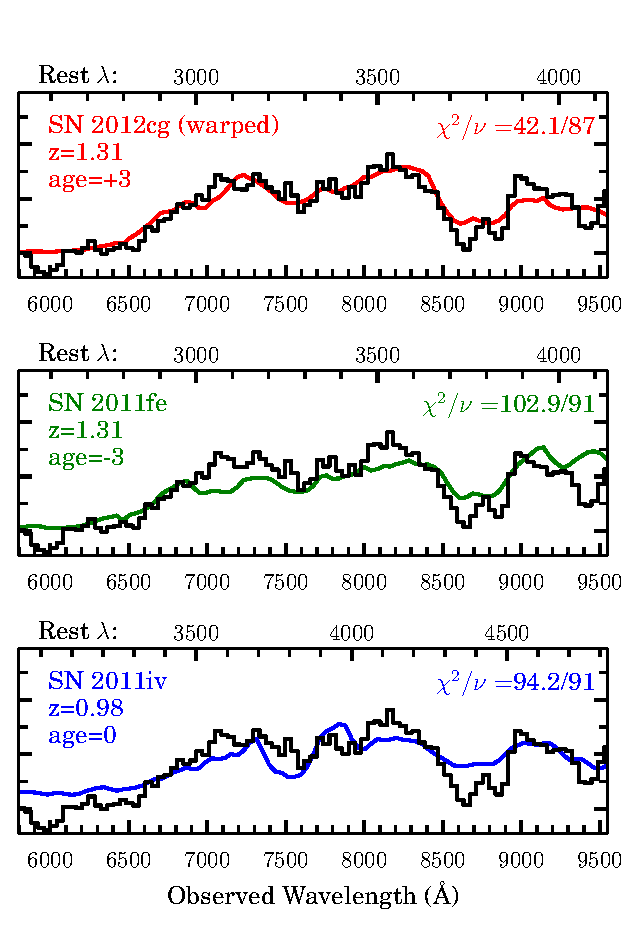
\includegraphics[width=\columnwidth]{FIG/specfit}
\caption{  \label{fig:SpecFit}
Redshift and age determination from spectral template matching to the
the SN \tomas\ maximum light spectrum.  The y axis plots flux in
arbitrary units, and the x axis marks wavelength in \AA\ with the
observer-frame on the bottom and rest-frame on the top.
The \tomas\ spectrum observed with the
HST ACS G800L grism is shown in black, overlaid with model fits
derived from a library of Type Ia templates that have extended
rest-frame UV coverage.  {\it Top}: The best match is at $z=1.31$ with
age=$+3$ days, from the normal Type Ia SN 2012cg template when using a
smooth 3rd-order polynomial to warp the shape of the template
pseudo-continuum.  When the templates are not warped, an acceptable
fit can be found with a normal Type Ia at $z=1.31$ (middle) or at
$z\sim1$ (bottom), although the latter is inconsistent with the host
galaxy redshift prior and the light curve. No \CCSN\ templates can
provide a statistically acceptable fit at any redshift, within the age
constraints imposed by the light curve.}
\end{center}
\end{figure}


A spectrum of SN \tomas\ was collected with the ACS G800L grism on
2014 June 4 and 7, when the SN was very near to its peak brightness.
The observations -- listed at the bottom of Table~\ref{tab:Photometry}
-- used 5 HST orbits from the FrontierSN program for a total
spectroscopic exposure time of $\sim$10 ksec.  The grism data were
processed and the target spectrum was extracted using the custom
pipeline employed by the Grism Lens Amplified Survey from Space
program (GLASS; PI:Treu, PID:13459). \textcolor{red}{Is there a
citation for this? or more to say here?}  

Figure~\ref{fig:SpecFit} shows the composite 1-D ACS grism spectrum,
combining all available G800L exposures, overlaid with SN model fits
that will be described below.  The spectrum is largely free of
contamination, because the orientation was chosen to avoid nearby
bright sources and the host galaxy is diffuse and optically faint.
Thus, the SN spectral features can be unambiguously identified, most
notably the red slope of the continuum and a prominent absorption
feature at $\sim$8700\AA.  However, the signal to noise ratio (S/N)
for the host galaxy spectrum was too weak to yield any additional
constraints on the host type or redshift.

As described below, we fit the SN \tomas\ spectrum in two steps.
First we determine a spectral classification -- and get a preliminary
estimate of the redshift and age -- using the SuperNova IDentification
(SNID) software \citep{Blondin:2007}.  Second, we refine the redshift
and age measurement using a custom Type Ia spectral template matching
program.

\subsection{Classification with SNID}
\label{sec:SNID}

The SNID program is designed to estimate the type, redshift, and age
of a SN spectrum through cross-correlation matching with a library of
template spectra.  To account for possible distortions in the broad
shape of the SN pseudo-continuum due to dust or instrumental
calibration effects, SNID divides each SED by a smooth cubic spline
fit. This effectively removes the shape of the SN pseudo-continuum to
leave behind a flat SED superimposed with spectral absorption and
emission features.  It is these features which drive the
cross-correlation fit, so the SNID approach is insensitive to the
overall color of the SED.  We used v2.0 of the SNID template library,
which includes template SEDs covering all Type Ia and Core Collapse
sub-classes, and has recently been updated with corrections and
improvements to the Type Ib/c templates \citep{Liu:2014}.

In SNID the goodness of fit is evaluated primarily through the {\it
rlap} parameter, which measures the degree of wavelength overlap and
the strength of the cross-correlation peak.  Typically, an {\it rlap}
value $>5$ is required to be considered an acceptable match.  

To match the SN \tomas\ spectrum we use conservative constraints on
age and redshift: limiting the age to $\pm$5 rest-frame days of peak
brightness and $0.8<z<1.8$, consistent with the SN light curve and
host galaxy photo-$z$.  With these constraints we find that the only
acceptable match is a normal Type Ia SN near $z=1.3$. The best match
has {\it rlap}$=8.7$, using the normal Type Ia SN 2005cf at $z=1.35$
and age=-2.2 rest-frame days before peak.  Within these constraints,
the best non-Ia matches all have {\it rlap}$<2.5$.

The {\tt SNID} library can generate an acceptable \CCSN\ match only
when we remove all age and redshift constraints, In this case the best
non-Ia match is the Type Ic SN 1997ef, which delivers {\it rlap}$=6.8$
at $z=0.51$ and age=47.3 rest-frame days past peak.  This is not as
good a fit as the best Type Ia models, is at odds with the host galaxy
redshift prior, and is strongly disfavored by the shape and colors of
the SN light curve (see Section~\ref{sec:PhotometricClassification}).  

From the preceding analysis, we conclude that \tomas\ is a Type Ia SN
at $z\approx1.3$.  At this redshift, the absorption at $\sim$8700\AA\
corresponds to the blended \ion{Ca}{2} H\&K features.
This \ion{Ca}{2} absorption is commonly seen in Type Ia SN spectra
near maximum light, although it is also prominent in the spectra of
Type Ib and Ic core collapse SNe (\CCSNe).  The red color of
the \tomas\ SED is qualitatively consistent with a redshift of $z>1$
-- although this information was not used by {\tt SNID} for the
template matching.  As we will see in Section~\ref{sec:PhotometricClassification},
this spectral classification of SN \tomas\ is reinforced by the
photometric information, which also supports classification as a Type
Ia SN at $z=1.3$.


\subsection{Spectroscopic Redshift}
\label{sec:SpecRedshift}

To refine the redshift and phase constraints on \tomas, we next fit
the spectrum with a custom spectral matching program that employs a
library of Type Ia SN SEDs.  This library is similar to the Type Ia
spectral set used by SNID, but also includes more recent SNe with
well-observed spectral time series that extend to rest-frame UV
wavelengths (e.g. SN 2011fe and 2014J).  We first use an approach
similar to the SNID algorithm: warping the pseudo-continuum of each
template spectrum by dividing out a 3$^{\rm rd}$-order polynomial to
match the observed SED of SN \tomas.  From this analysis we find
results that are consistent with the SNID fits: a redshift of
$z=1.31\pm0.01$ and a phase of $0\pm3$ rest-frame days. The
best-fitting spectral template is the normal Type Ia SN 2012cg, shown
in the bottom panel of Figure~\ref{fig:SpecFit}, which has $\chi^2$
per degree of freedom $\nu$ equal to 42.1/87.

Finally, we repeat the fitting, but without any warping of the
templates to account for differences in the continuum shape.  In this
iteration we only allow each template SED to be scaled in flux
coherently at all wavelengths.  As shown in Figure~\ref{fig:SpecFit},
we again find that the \tomas\ SED can be matched by a normal Type Ia
SN (SN 2011fe) at redshift $z=1.31\pm0.01$.  Without the continuum
warping, an alternative fit also arises: the normal Type Ia SN 2011iv
at $z=0.98\pm0.01$. Formally, this match provides a slightly better
fit to the unwarped \tomas\ spectrum, although the fit is notably poor
at $\sim8700$\AA\ where the most significant absorption feature is
found. Furthermore, a redshift $z\sim1$ is at odds with the host
galaxy photo-z ($1.5\pm0.2$), and we will see in the following section
that the photometric data is incompatible with a normal Type Ia SN at
$z\sim1.0$.

Setting aside the $z\sim1$ solution, all other template matches
provide a consistent redshift constraint of $z=1.31\pm0.01$,
regardless of whether the templates are warped to match the SN \tomas\
continuum shape.  The inferred age from these fits is $0\pm3$
rest-frame days from peak brightness, which is also consistent with
the observed light curve.


\section{Photometric Classification}
\label{sec:PhotometricClassification}

Relative to other SNe at $z>1$, the SN \tomas\ light curve was
unusually well sampled at rest-frame ultraviolet wavelengths, due to
the rapid cadence of the HFF imaging campaign. These ACS observations
therefore provide a tight constraint on the time of peak brightness
and the evolution of the SN color.  Supplemental observations with the
WFC3-IR camera provided critical rest-frame optical photometry,
enabling a measurement of the apparent luminosity distance through
light curve fitting.

As a check on the spectral classification of SN \tomas\
(Section~\ref{sec:SNID}), we independently classified the SN using a
Bayesian photometric classifier.  This classification code uses the
{\tt sncosmo} software
package\footnote{\url{http://sncosmo.github.io/}} to simulate SN light
curves at a range of redshifts and evaluate the classification
probability using traditional Bayesian model selection \citep[as
in][]{Jones:2013,Rodney:2014,Graur:2014,Rodney:2015}.  In this
analysis we represent normal Type Ia SNe with the SALT2
model \citep{Guy:2010}, and \CCSNe\ with 42 discrete templates (26
Type II and 16 Type Ib/c) drawn from the template library of the
SuperNova Analysis software package \citep[SNANA,][]{Kessler:2009a}.
Likelihoods are defined by comparing the observed fluxes to model
predictions in all passbands where the model is defined.  In practice,
this means we exclude the F435W and F606W bands, which are too blue
for our models at $z>1$. 

The \CCSN\ models have free parameters for date of peak brightness
($t_{\rm pk}$), amplitude, and redshift ($z$). Due to the expected
impact of gravitational lensing magnification, we do not include any
prior on the intrinsic luminosity for any SN sub-class.  We also do
not assign a prior for the SN redshift. This allows our photometric
analysis to provide an independent check on the host galaxy photo-$z$
and spectroscopic redshift (Sections~\ref{sec:HostGalaxy}
and \ref{sec:SpecFit}).

For Type Ia SNe, the SALT2 model has two additional parameters that
control the shape ($x_1$) and color ($c$) of the light curve.  We use
conservative priors here, defined to encompass a range of Type Ia SN
shapes and colors that is broader than typically allowed in
cosmological analyses \citep[see
e.g.][]{Kessler:2009b,Sullivan:2011,Rest:2014}. For $x_1$ the prior is
a bifurcated Gaussian distribution with mean $\bar{x}_1=0$, dispersion
$\sigma_{x_1}^+={0.9}$ and $\sigma_{x_1}^-={-1.5}$.  The prior for the
color parameter $c$ has $\bar{c}=0.0$, $\sigma_c^-=0.08$, and
$\sigma_c^+=0.54$.  The $c$ parameter in SALT2 combines intrinsic SN
color and extinction due to dust, so the large red tail of this
distribution allows for the possibility of several magnitudes
of dust extinction along the \tomas\ line of sight.

We also assign a class prior for each of the three primary SN
sub-classes (Type Ia, Ib/c, and II), using a fixed relative fraction for
each sub-class as determined at $z=0$ by \citet{Smartt:2009}
and \citet{Li:2011a}.  A more rigorous classification would extrapolate
these local SN class fractions to higher redshift using models or
measurements of the volumetric SN rate.  For simplicity, we do not
vary the class priors with redshift, and in practice these priors do
not have any significant impact on the resulting classification.

The final photometric classification probability for SN \tomas\ is
$p({\rm Ia}|{\bf \rm D})=1.0$, with the classification
probability from all \CCSN\ sub-classes totaling less than $10^{-100}$.  The
marginal posterior distribution in redshift for the Type Ia model is
sharply peaked at $z=1.36\pm0.02$, which is $<2.5\sigma$ from
the spectroscopic redshift of $z=1.31\pm0.01$ derived in
Section~\ref{sec:SpecRedshift}.  The time of peak brightness is also
tightly constrained at $t_{\rm pk}=56816.0\pm0.2$, which means the
spectroscopic observations were collected within 2 rest-frame days of
the epoch of peak brightness, consistent with our spectroscopic
analysis. 


\section{Light Curve Fitting}
\label{sec:LightCurveFitting}

With the spectroscopic type and redshift securely defined as a normal
Type Ia SN at $z=1.3$, we now turn to fitting the light curve with
Type Ia templates to measure the distance modulus.  Here we use two
independent light curve fitters: first the SALT2 model described
above, and then the MLCS2k2 model from \citep{Jha:2007}.

\subsection{SALT2 Fit}
\label{sec:SALT2Fit}

in \citep{Patel:2014}:   $\alpha=1.367\pm0.086$,
$\beta=3.179\pm0.101$, $M=-19.12\pm0.03$.

For the SALT2 Type Ia model one can define a shape- and color-corrected apparent
B-band magnitude using 
$m_{\rm B}^\prime = m_{\rm B} + \alpha x_1 - \beta c$. 

For the SALT2 model we fix the model parameters to the values
derived in the \citet{Rest:2014} analysis of the Pan-STARRS1 SN sample:
$\alpha=0.147$, $\beta=3.13$, $M_B=-19.34$.

Comparing salt2 color to Av \citep{Kessler:2009b}:
$c = (0.464 ± 0.021)AV − (0.121 ± 0.014)$

from \citet{Patel:2014}:
``Finally, to ensure a consistent zeropoint between the SALT2 and
MLCS2k2 distance moduli, we applied both methods to a sample of SDSS
Supernova Survey SNe Ia from Holtzman et al. (2008) and Kessler et
al. (2009a). We added a zeropoint correction of 0.20 mag to the
distance moduli reported by SNANA in the MLCS2k2 fit (dmMLCS2k2), to
put them on the same scale as the SALT2 distances (dmSALT2).''


\subsection{MLCS2k2 Fit}
\label{sec:MLCS2k2Fit}

As in \citep{Patel:2014}.


$R_v$ fixed to 1.9. 

for Rv = 1.9, the calibrated distance is: $\mu = \mu_{\rm mlcs}-0.2006$. 

\begin{figure}
\begin{center}
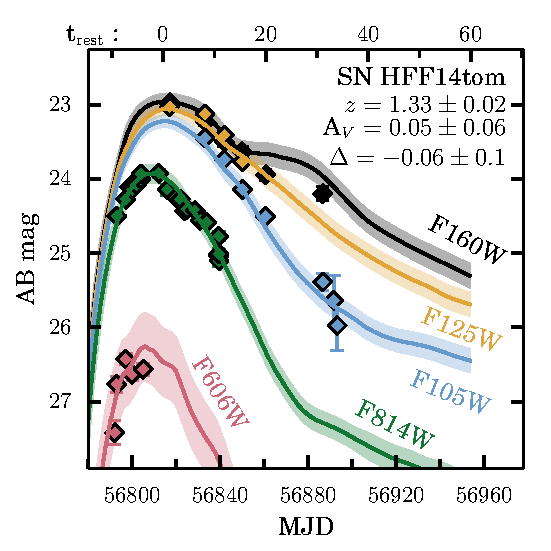
\includegraphics[width=0.49\textwidth]{FIG/lcfit_mlcs2k2_ABmag}
\caption{  Light curve fit using MLCS2k2. 
\label{fig:mlcsfit} }
\end{center}
\end{figure}

\section{Lensing Magnification}
\label{sec:LensingMagnification}


\subsection{Direct Magnification Measurement}
\label{sec:DirectMagnificationMeasurement}


\begin{figure}
\begin{center}
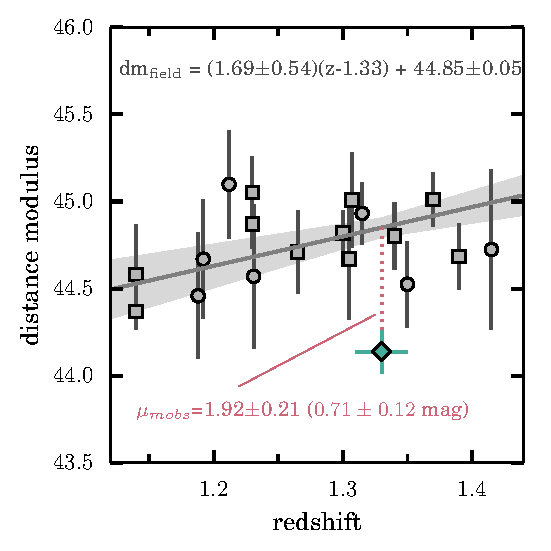
\includegraphics[width=\columnwidth]{FIG/magnification_measurement}
\caption{ Deriving the magnification from comparison to field SN
\label{fig:magmeasure} }
\end{center}
\end{figure}

\subsection{Comparison to Model Predictions}
\label{sec:ComparisonToModelPredictions}


1) All of the lens models predict a higher magnification than we observe, some with discrepancies >5 sigma.  This suggests a systematic bias inherent to all the models -- at least for this particular line of sight. 

2) the addition of new lensing constraints from the HFF data does not reduce the tension.  From both of the most recent models (Jauzac+ 2014 and Lam+ 2014) the predicted magnification is still significantly higher than the observed. 

3) The pre-HFF models that come closest to matching the observed magnification are the Zitrin-NFW and Merten models (also the Williams model, though it has very large uncertainties).  Those happen to be two models that relax or remove the assumption of light-traces-mass.  


\begin{figure}
\begin{center}
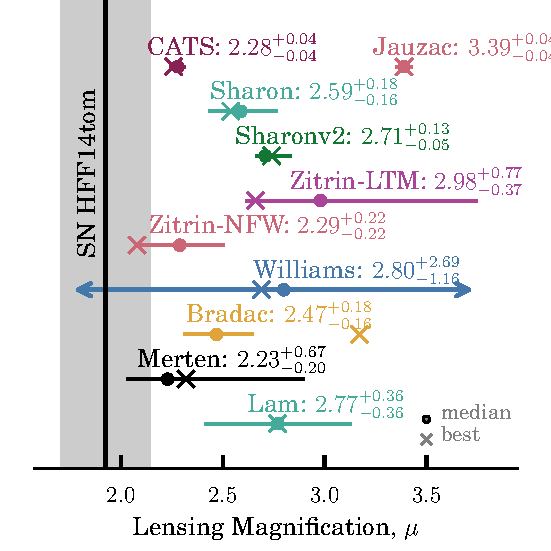
\includegraphics[width=\columnwidth]{FIG/lensing_test}
\caption{ 
Comparison of the observed lensing magnification to predictions from
lens models.
\label{fig:lensingtest} }
\end{center}
\end{figure}


\section{Discussion}

Possible sources for the bias. 

Implications for the systematic error budget of high-z lenses.

Design elements for a survey to build a bigger sample : HST GO, Snapshot, ground-based.

\bigskip


{\bf Acknowledgments:}

We are very pleased to thank the Hubble Frontier Fields team at STScI
for their substantial efforts to make the HFF program successful.  In
particular, thanks are due to Matt Mountain for the allocation of
discretionary orbits for the HFF program; to Jennifer Lotz, Norman
Grogin and Patricia Royle for accommodations in strategy and
implementation to make the FrontierSN program possible; and to Dan Coe
for curating the excellent and accessible lens model comparison tools.
We also must thank the CLASH team, led by Marc Postman, for
observations, catalogs, and high level science products that were of
significant value for this analysis.

Financial support for this work was provided by NASA through grants
HST-HF-51312 and HST-GO-13386 from the Space Telescope
Science Institute, which is operated by Associated Universities for
Research in Astronomy, Inc., under NASA contract NAS 5-26555.  Support
for this research at Rutgers University was provided in part by NSF
CAREER award AST-0847157 to SWJ.  The Dark Cosmology Centre is
supported by the Danish National Research Foundation.


{\it Facilities:} \facility{HST (WFC3)}
\smallskip

\bibliographystyle{apj}
\bibliography{bibdesk}

\end{document}

